\documentclass{article}
\usepackage{cs6850}

\renewcommand\maketitle{
\begin{flushleft}
{%
\large{%
Benjamin Greenman,
Hersh Mehta
\hfill
CS6850: Topic Proposal
\\\texttt{\{blg59, hpm36\}} \hfill \today
}}\\
\hrulefill
\end{flushleft}
}

\begin{document}
\maketitle

%% Quick paper, about 2 pages in length, what we're planning to do for the project.
%% If your project is based on your reaction paper, then you don't need to repeat things you've said in the reaction paper -- 
%% it's enough to describe how you're planning to turn the ideas from the reaction paper into a larger project.

\subsection*{Topic}
Our plan for the course project is very similar to the plan we presented in the reaction paper. 
We intend to explore the phenomena of herding in high-frequency trading (HFT) markets, attempting to understand and model the behavior. 
To do this, we will utilize simulated and collected data, developing a model and testing its hypothesis against real-world behaviors. 

%% \subsubsection*{Background}
Herd behavior in stock markets is a fairly well-studied subject.
The earliest relevant literature dates back to the late 1980's \cite{bikhchandani}, and since then a number of experiments and theoretical models have observed and characterized the behavior.
These results are far from authoritative, but they established at least that herding exists and offer reasonable suggestions for modeling the phenomena.
However, high-frequency trading has recently overhauled our conception of a securities market, and little to no published literature explores this phenomena.
We attempt to correct this deficiency.

\subsection*{Hypothesis}
Building upon the results of existing models and our own intuition and experiences regarding high-frequency markets, we have a few hypotheses about high-frequency trading that our project will test.
First, we assume that herding does in fact exist in HFT markets.
Significant evidence points to the existence of herding in traditional financial markets \cite{scharfstein1990herd,grinblatt1995momentum,trueman1994analyst,devenow1996rational,golec1997herding,lin,lakonishok1992impact,sias2004institutional}.
Additionally, researchers have noted cases in which there are monetary incentives for herding, such as minimizing risk and hedging bets to address a lack of private data.
Thus we expect trading algorithms to identify and take advantage of opportunities presented by herding. 

Second, and more crucial, we hypothesize that trading volume has a major influence on herding. 
The larger quantity traded in an exchange, the greater likelihood that other investors in the market will herd according to this decision.
This we believe will have a larger impact on herd behavior than any other metric, including trade frequency.
Ceteris parebis, we expect a few exchanges totaling quantity $Q$ to have a lesser effect on predicting herd behavior than one large exchange of the same quantity.

This hypothesis has not, so far as we know, been tested in the existing literature, and certainly not for HFT data.
Hence this is what we seek to measure: by assuming that volume plays the most significant role, we hope to develop a model that successfully predicts herding.

\subsection*{Protocol}
We plan to test our hypothesis in two stages, through simulation and data.
First, we will develop a new herding simulation, building upon those given in other work.
Next we will use data collected through the Interactive Broker API to test our hypothesis and model. 

\subsubsection*{Simulation}
We focus is on the model presented by Boortz et~al., which had in turn built off the models of Sias and Park \& Sabourian \cite{boortz,sias2004institutional,park2011herding}.
There are a number of assumptions made by this model that we take issue with. 
Foremost is their choice of conditional probability for deterimining investor behavior, which we will alter to account for the volume of each exchange.
Additionally, we are considering techniques for indexing investors to better model their behavior and removing the noise traders they introduced to the simulation.
The idea of noise traders is counterintuitive\textemdash participants do not trade blindly, though they may be resistant to herding.
Hence we introduce an alternate component where Boortz had used noise traders. 

Our goal is not to complicate the existing model or to introduce more variables.
Rather we want a model that more appropriate describes real-world interactions. 
Simulation in hand, we will use it to determine how at what quantity individual trades become large enough to significantly influence herding in HFT markets.

\subsubsection*{Data}
The Interactive Broker API will be our primary source of data. 
Other sources we have considered are either of poor quality, without quantities or at low frequencies, or too expensive given the scope of this project.
However Interactive Broker presents a challenge in that we may only gather data for one stock at an interval. 
We may collect for different stock on varying weeks, days, or hours, but cannot simultaneously gather data on multiple securities.
This is not so great a barrier\textemdash in fact thinking on how to best leverage data on few securities has already helped focus our efforts\textemdash yet it hinders our potential.
Hence we continue to seek alternate data sources to supplement our experiment.

%% What to do, use the graph
With this data, we intend to construct a graph similar to the one presented by Almgren in Figure \ref{fig:almgren} (see Appendix) in his presentation on interest rate futures \cite{almgren}.
Namely, we plot the best bid and ask prices along with the current quantity-weighted average.
In addition, we will note where large-quantity trades occur (using the quantities identified in our simulation), and inspect where these points are in relation to high-slope areas of the graph.
Our suspicion is that the best bid and asks will shift corresponding to these large-quantity trades.

%% \subsection*{Conclusion}

Looking forward to finding and sharing some results!

\bibliographystyle{amsplain}
\bibliography{topic-proposal}

\newpage

\section*{Appendix}

\begin{figure}[h]
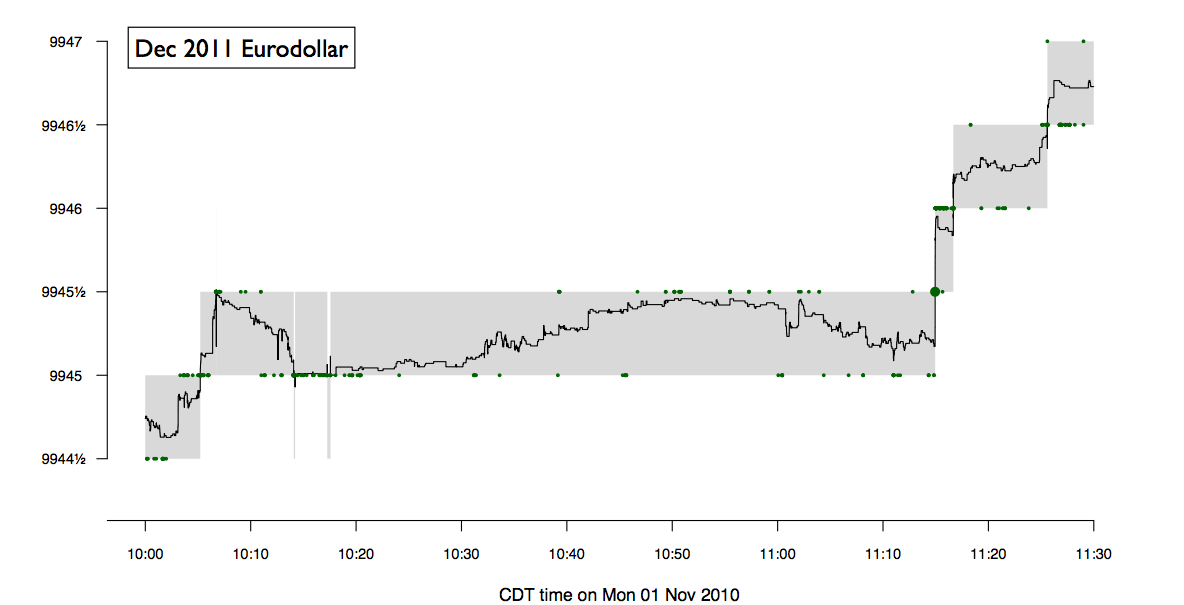
\includegraphics[width=\textwidth]{almgren.png}
\caption{Plot of best bid and ask prices (difference is shaded area) and quantity-weighted average bids.}
\label{fig:almgren}
\end{figure}

\end{document}
